%%%%%%%%%%%%%%%%%%%%%%%%%%%%%%%%%%%%%%%%%%%%%%%%%%%%%%%%%%%%%%%
%
% Welcome to Overleaf --- just edit your article on the left,
% and we'll compile it for you on the right. If you give 
% someone the link to this page, they can edit at the same
% time. See the help menu above for more info. Enjoy!
% 
%%%%%%%%%%%%%%%%%%%%%%%%%%%%%%%%%%%%%%%%%%%%%%%%%%%%%%%%%%%%%%%
%
% For more detailed article preparation guidelines, please see:
% http://f1000research.com/author-guidelines and http://f1000research.com/data-preparation

\documentclass[9pt,a4paper]{extarticle}
\usepackage{f1000_styles}

\usepackage{listings}
\usepackage{color}
\usepackage[dvipsnames]{xcolor}
\usepackage{nameref}
\usepackage{tabularx}
\usepackage{float}

\usepackage{enumitem}
\setlist[enumerate,1]{start=0} % only outer nesting level

\definecolor{string}{rgb}{0.3,0,0}


\lstdefinestyle{json}{
  basicstyle=\normalfont\ttfamily,
  tabsize=2,
  showstringspaces=false,
  breaklines=true,
  language=C,
  stringstyle=\color{string},  
  xleftmargin=.25in,
}

\begin{document}
\pagestyle{front}

\title{\textit {Grassroots}: software infrastructure for sharing scientific services and data}
%\titlenote{The title should be detailed enough for someone to know whether the article would be of interest to them, but also concise. Please ensure the broadness and claims within the title are appropriate to the content of the article itself.}
\author[1]{Simon Tyrrell*}
\author[1]{Xingdong Bian}
\author[2]{Paul A. Wilkinson}
\author[2]{Keith J. Edwards}
\author[1]{Robert P. Davey}
\affil[1]{Earlham Institute,
Norwich Research Park,
Norwich,
NR4 7UG,
UK.}
\affil[2]{School of Biological Sciences,
University of Bristol,
Bristol,
UK.}

\maketitle

* To whom correspondence should be addressed. Email: simon.tyrrell@earlham.ac.uk

\thispagestyle{front}

%Please list all authors that played a significant role in developing the software tool and/or writing the article. Please provide full affiliation information (including full institutional address, ZIP code and e-mail address) for all authors, and identify who is/are the corresponding author(s).



\begin{abstract}

Since the dawn of the internet, scientific analysis software has been able to be run as online services. These can range from tools such as BLAST\cite{Camacho:2008}, SwissDock\cite{Grosdidier2011SwissDock}.
Historically, these would have been "single use" tools, providing access to one tool or package of tools in order to analyse some small datasets. Given the subsequent explosion of datasets and new tools to analyse them, many scientific services are now provided on high-powered web servers and many offer application programming interfaces (APIs) to allow them to be called programmatically rather than requiring human interaction.

As an increasing number of online services become available and popular, the issue of how to share data between the services becomes prevalent. The data that they input and output can be in differing data formats and be difficult and time-consuming for a user to reconcile the results together. Similarly  .These are the primary issues that we are developing the Grassroots infrastructure to solve.

%(Might need a bit more intro as to why we need Grassroots - "The problem with many diverse/siloed data resources/analysis services is... Therefore we are developing Grassroots to ... "). 

The Grassroots API is an infrastructure to allow both these services and associated data to be shared between geographically separated servers allowing users access to these distributed services transparently without having to have separate concurrent sessions with each of these servers.

The Grassroots architecture provides a consistent framework for easy development of services and methods for integrating these services together to generate as many knowledge interconnections as possible.

%Abstracts should be up to 300 words and provide a succinct summary of the article. Although the abstract should explain why the article might be interesting, care should be taken not to inappropriately over-emphasise the importance of the work described in the article. Citations should not be used in the abstract, and the use of abbreviations should be minimized. 

\end{abstract}

\clearpage
\pagestyle{main}
\section*{Introduction}

Many scientific services are now provided on web servers and many offer application programming interfaces (APIs) to allow them to be called programmatically. 
However, most of the time, these services are not designed to be easily integrated with other services meaning that a user needs to access each service individually, saving and potentially having to convert the results from one service to be used in another. 
Another situation is that if multiple servers offer similar services on differing sets of data, \textit{e.g.} BLAST searches on different databases, keyword searches, \textit{etc.}, a user would have to run each service individually, having to ensure that input parameters are identical so that the comparison of results is valid. 

The Grassroots Infrastructure project aims to create an easily-deployable suite of computing middleware tools to help users and developers gain access to scientific data infrastructure that can easily be interconnected.

With the data-generative approaches that are increasingly common in modern life science research, it is vital that the data and metadata produced by these efforts can be shared and reused. 
The Grassroots Infrastructure project wraps up industry-standard software tools along with our own custom open-source software tools to give a consistent API that can be federated with others in terms of both data and services. 
This means institutions and groups can deploy a simple lightweight software suite, locally or as a virtual machine, to expose institutional data, connect up any existing data services, and federate their instance of Grassroots with other remote instances.

One of the major aims of the Grassroots Infrastructure is to allow users to share their wheat data, although it is by no means organism-specific, as easily and seamlessly as possible. 

An important part of this is the linking of data and services together as much as possible. Similar to the cohesion between web pages, images, maps, \textit{etc.} as part of a Google search, the Grassroots system attempts to link together data so that, for a given pathogen for example, any data from samples are linked with any academic papers into the topic, \textit{etc.}
This is achieved by using Linked Data and JSON-LD with well-documented ontologies and schemas allowing data to be marked up for reuse as effectively as possible.

%%%%%%%%%%%%%%%%%%%%%%%%%%%%%%%%%%%%%%%%%%%%%%%%%%%%%%%%%%%%%%%%%%%%%%
%%%% Currently our mark up is for the pathogenomics and hopefully %%%%
%%%% Cerealsdb snp services. If the pathogenomics stuff is in a   %%%%
%%%% separate paper, there won't be that much to mention here.    %%%%
%%%% Any thoughts?
%%%%
%%%% Rob 20160407:
%%%% We still need to make sure we address why Grassroots is
%%%% needed and the reasoning behind why we did what we did.
%%%% The intro shouldn't have anything about our specific use cases.
%%%%%%%%%%%%%%%%%%%%%%%%%%%%%%%%%%%%%%%%%%%%%%%%%%%%%%%%%%%%%%%%%%%%%%


\section*{Methods}%Abstracts should be up to 300 words and provide a succinct summary of the article. Although the abstract should explain why the article might be interesting, care should be taken not to inappropriately over-emphasise the importance of the work described in the article. Citations should not be used in the abstract, and the use of abbreviations should be minimized. 



%%%%%%%%%%%%%%%%%%%%%%%%%%%%%%%%%%%%%%%%%%%%%%%%%%%%%%%%%%%%%%%%%%%%%%

%%%% Currently our mark up is for the pathogenomics and hopefully %%%%

%%%% Cerealsdb snp services. If the pathogenomics stuff is in a   %%%%

%%%% separate paper, there won't be that much to mention here.    %%%%

%%%% Any thoughts?

%%%%

%%%% Rob 20160407:

%%%% We still need to make sure we address why Grassroots is

%%%% needed and the reasoning behind why we did what we did.

%%%% The intro shouldn't have anything about our specific use cases.

%%%%%%%%%%%%%%%%%%%%%%%%%%%%%%%%%%%%%%%%%%%%%%%%%%%%%%%%%%%%%%%%%%%%%%



\subsection*{Implementation}
%For software tool papers, this section should address how the tool works and any relevant technical details required for implementation of the tool by other developers.  

The Grassroots infrastructure works as a server-client application typical of existing web services. 
Rather than working as a centralised system, the Grassroots infrastructure uses a distributed architecture where each server is a node that can be connected together and share their data and services. 
From a user's point of view, these shared resources appear as they all exist upon the server that the user is connected to.

There are two parts to the Grassroots infrastructure; the schema that defines the messages that are used for the server-client and server-server communication, and the software tools constituting the server, services, support libraries and clients.

All of the server-client and cross-server communication is performed using JSON\cite{JSON} messages that conform to the Grassroots schema. 
These messages form a specification and any software tools that are able to interpret these messages correctly can be used. 
This is analogous to the consumption of HTML content by a variety of different web browsers, servers, command line tools, \textit{etc.} 
These message describes services, parameters and results of running services and are fully self-describing so that no prior knowledge of the service is needed by the receiver of these messages to be able to understand all of the information described in these messages. 

The key part of being able to use the Grassroots architecture is being able to receive and respond to these JSON messages, so software can be implemented in any programming language or using any compliant tools.
The software libraries that are currently within the Grassroots infrastructure are mainly written in C/C++ or Java for the server-based tools and C/C++ or javascript for the client applications.

A schematic of the Grassroots architecture is shown in Figure \ref{fig:httd_grassroots}. The currently available Grassroots server software can be easily integrated into an Apache HTTP Server (httpd)\cite{httpd} by loading a custom Grassroots httpd module and configuration file into httpd. By using httpd, the server can take advantage of all of the functionality and security that httpd provides.  

The next section of the schematic shows the set of libraries that give much of the underlying functionality of the Grassroots infrastructure. These libraries include common code for various tasks such as converting the various system components to and from their schema representations, accessing data on local, remote and cloud-based storage systems, creating jobs for High Performance Computing (HPC) clusters, \textit{etc.}

The code modules that provide the scientific analysis are called services.
Although the actual functionality provided by each service can vary, \textit{e.g.} scientific analysis, text mining, similarity searching, \textit{etc.}, the methods of transmitting the required information to run each service and returning their results can be standardised through these JSON fragments. 
Each service conforms to the same API which allows the system to query its capabilities such as \textit{e.g.} its name, description, an optional web page describing the service in greater depth, its parameters, which also have names, descriptions, default values, \textit{etc.}, run the service, query the status of its jobs, \textit{etc.} 
So any code that conforms to this API can be added to the system as a service.


\subsection*{Services}

Services can run in two different ways. The first mode is synchronously where the service runs to completion before returning any results to the user. All of the resources that the service requires to run the job can be released as it sends the response back
The second approach is that a service can be run asynchronously where it starts its work and returns immediately. The job then continues and the user can send a message to periodically check whether the job has completed successfully or not. With this approach any required resources need to be accessible between different requests. Given that httpd can  run as a multi-threaded and/or multi-process system, any data that needs to be persistent, \textit{i.e.} stored between requests, has to be adaptable to any httpd runtime configuration.

So the Grassroots system has an interface for interacting with asynchronous jobs which is a module called JobsManager which deals with sharing persistent data between requests. There are currently two implementations of this. The first is for Apache httpd web server in a module called the APRJobsManager, since it uses the Apache Portable Runtime (APR) libraries. The second instance uses the Grassroots MongoDB libraries to store the job details in a MongoDB database.
All of the needed data to be able to recreate and access the job between processes and/or threads is stored in this module.

The available JSON keys for describing parameters are show in tables \ref{tab:parameter} and \ref{tab:parameter_types}.

%% ((need a complete list. etc is a cop out! :) ) 
%% ST - Fair cop! Added tables for parameter details 

In this way, any changes to a service such as adding a parameter or changing default values need only be made by the service, and the server and the client will automatically take these amendments into account.

One of the goals of the Grassroots architecture is to allow users to use distributed services seamlessly.
Grassroots-enabled servers can be connected together to allow users access to all of the combined services, regardless of which server they connect to. 

As well as connected Grassroots servers being able to combine their list of services, the individual services themselves can also be integrated. 
For example, separate servers can run similar services which access differing datasets and these two services can be passenger presented to user as a single service with access to the combined list of datasets as shown in Figure \ref{fig:client_view}. 
This means that the user only has to enter their chosen parameters once rather than having to go each instance of the service individually and duplicate their parameter choices. 

\subsubsection*{Data}

As well as connecting both internal and external services together, the Grassroots architecture also can be use federated data. Data access, such as reading and writing data, is abstracted and can be located on an accessible filesystem or an HTTP(S) URI. 
There is also partial support for accessing resources located on a Dropbox\cite{Dropbox} share and within Integrated Rule-Oriented Data System (iRODS)\cite{2007AGUFMIN13B1214R}. iRODS is a data management system that virtualizes where data is stored and allows the adding of metadata key-value pairs to any of the objects stored within it. It also allows different remote iRODS storage areas to federated together so that a user can access all joined areas transparently.


\subsubsection*{Service creation}

There are two types of services within a Grassroots system; middleware services and JSON services.

Middleware services can be written in any language as long as they can support the input and output of JSON messages. All of the services currently in the Grassroots system are written in C/C++ or Java though any other JSON-aware language can be used if preferred. These services have a standard structure with a set of callback functions that need to be filled in to \textit{e.g.} expose the service's name, its parameters, run the service, get its results, \textit{etc.} and these methods have the same function signatures regardless of the underlying service functionality. 

The only information that the Grassroots server knows about these services is gained from the querying the services themselves via their callback functions, the server has no prior details about any of the services. The advantages of this is that if a service needs changing, \textit{e.g.} a new parameter adding, changing default values, \textit{etc.} then they just need to be changed in the service configuration and the changes will automatically get picked up any servers or clients accessing the service. 

Services can also be created without the need to write a program in a lower-level language. It is also possible to define a service, \textit{e.g.} a web-based search service, simply by filling in a JSON-based template file and loading it into a Grassroots instance. 
One of the libraries that comes with the Grassroots system is a library for integrating an external representational state transfer (REST) web service as a Grassroots service and a complete example is shown in Figure \ref{fig:json_service}. The key sections of this template for accessing the REST service are:

\begin{lstlisting}[style=json]
"plugin": "web_search_service"
\end{lstlisting}
This template specifies the plugin library to use, web\_search\_service.

\begin{lstlisting}[style=json]
"uri": "http://agris.fao.org/agris-search/searchIndex.do",
"method": "GET",
"parameter_set": {
  "parameters": [{
  "param": "query",
     ....
\end{lstlisting}
This specifies the URI to submit the request to, the HTTP protocol to use and the name of the input parameter to use.

\begin{lstlisting}[style=json]
"link_selector": "li.result-item h3 a"
\end{lstlisting}
This specifies the CSS selector to use to extract the results from the REST web service's response.

\subsubsection*{Example services}

The middleware services currently available are:

\begin{description}

\item [BLAST Search] This service allows users to perform BLAST searches against available databases.
It is possible to run the user's requests using BLAST locally on the Grassroots server or it can use LSF-\cite{lsf} or SLURM-based\cite{yoo2003slurm} schedulers on high performance computing clusters. 
This service has the capability to be merged with external Grassroots servers that are
also running a BLAST service. When merged, the user will be presented with a single instance of a BLAST
service with a list of all of the available databases on the connected servers. This is described in more depth in the "Use Cases" section. 

% had to explicitly use "Use Cases" as \nameref{sec:usage} doesn't appear to work

\item [Ensembl] This services access a subset of the REST API available at http://ensemblgenomes.org\cite{kersey2016ensembl} and is currently focused upon the sequence-based functionality.

\item [iRODS] The integration of the Grassroots system with iRODS goes further as well with the addition of an iRODS search service. 
This allows the user to see all potential metadata keys and their range of values and create a search query accordingly.
It also allows a free-text search across all of the metadata values throughout the system, regardless of the key. 
Both of these searches are enhancements to iRODS that come specifically from the Grassroots service.

\item [Scaffold] This service uses the SamTools\cite{li2009sequence} code to get a complete scaffold regions from indexed reference sequences. This is accessible from results of a BLAST search when using the web-based client.


%%%%%%%%%%%%%%%%%%%%%%%%%%%%%%%%%%%%%%%%%%%%%%%%%%%%%%
%%% TODO: Add the bristol snp and contig services. %%%
%%%%%%%%%%%%%%%%%%%%%%%%%%%%%%%%%%%%%%%%%%%%%%%%%%%%%%

\end{description}

The JSON services currently available all connect to web-based search engines as described below:

\begin{description}
\item [Agris] AGRIS\cite{Agris} (International System for Agricultural Science and Technology) is a publicly accessible database with access to bibliographic information for agricultural science and technology globally.
\item [BASE] The Bielefeld Academic Search Engine\cite{Pieper2015} is a search engine for open access academic resources.
\item [f1000] F1000Research\cite{f1000} is a publishing platform for open science with a focus on immediate publication of articles, posters and slides.
\end{description}


\subsubsection*{Keyword-aware services}

A Grassroots system can receive a request to run some of its service with a given set of parameters or it can run a global keyword search, analogous to the Google search box. When the system runs a keyword search, there are two ways in which services can process a given keyword value
The first is based upon the fact that one of the datatypes that a service's parameter can be is a keyword type. So for all of a service's parameters that are specified as being keyword parameters, their values are set to the designated value and the service is automatically ran and the results returned to the user. 
The second approach is when a service recognizes that the keyword value is relevant but the value is not enough on its to run the service with and extra information is needed. So the service is sent back to the client application that the user is using with its parameters partially filled in for the user to complete and run if desired. An example of this is the BLAST service which reads through the names and descriptions of each of each of its databases to check for a given keyword value. If there is a match, then the service is returned to the client with the appropriate databases selected.

% TODO: describe ontology support and linked data

\subsection*{Operation}
%This part of the methods should include the minimal system requirements needed to run the software and an overview of the workflow for the tool for users of the tool.

Any server of client software that can process the JSON-based Grassroots messages can become part of the Grassroots ecosystem. 



Currently there is a Grassroots module to run a Grassroots server under httpd 2.4.x and higher. 

For advanced users to submit requests, any tool that can submit the JSON-based messages using an HTTP(S) protocol will suffice such as \textit{e.g.} curl\cite{curl}, \textit{etc.} 

A web-based client is also available which uses Java\cite{Java} and javascript. There is also a Qt-based\cite{qt} desktop client is also provided for users. This builds the entire user interface (UI) dynamically purely from the service descriptions received from a Grassroots server, choosing appropriate parameter editors depending upon the datatypes of the services' parameters. 

The initial versions of the Grassroots system and the Qt-based desktop client are available for Linux, however since all of the platform-specific code is contained within three small modules, porting to other platforms is trivial and versions for Windows and OSX will follow shortly.

%%%%%%%%%%%%%%%%%%%%%%%%%%%%%%%%%%%%%%%%%%%%%%%%%%%%%%%%%%%%%%
%%% TODO: DRMAA %%%
%%%%%%%%%%%%%%%%%%%%%%%%%%%%%%%%%%%%%%%%%%%%%%%%%%%%%%%%%%%%%%


%\section*{Results} % Optional - only if novel data or analyses are included
%This section is only required if the paper includes novel data or analyses, and should be written as a traditional results section.

\section*{Use Cases} \label{sec:usage} % Optional - only if NO new datasets are included

Consider the situation where a user wishes to run computational experiments across multiple data sources which are accessed via different servers. 
This common scenario requires the user to access each of these servers individually. For valid comparisons, the user might well need to use the same set of input parameters for each job upon these servers and the results would then need to be collated together. Both of these tasks can be prone to human error and also time consuming. 

The Grassroots architecture has two features to solve these problems. The first is that Grassroots servers can be connected together so that all of their services and data can be shared between them. This means that a user connecting to one of these servers will access to the services and data on all of the connected servers.

The second feature of the Grassroots architecture is its ability to merge the facilities of similar services running on separate servers into a single amalgamated service. This means that rather than multiple copies of the same service, one for each of the connected Grassroots servers with all of the problems mentioned above, 
For example, if the service performs computational tasks on some datasets, then the amalgamated service would have all of the datasets available for the connected servers' copies of this service. From a user’s viewpoint, it will appear as though the services and all of their combined facilities are running as a single service. 

An example of this has been set up between separate Grassroots instances at the Earlham Institute and at the Cereal Genomics lab at the University of Bristol allowing a BLAST service to run against an amalgamated set of databases. 
Each institution has its own set of BLAST databases and rather than have to copy these files between the two institutions and deal with issues such as synchronisation of any changes or updates to these files, the servers are connected using the Grassroots API. A user can connect to either institution and run a BLAST query against any selection of the databases available at both institutions. 
This means that instead of having to run two separate jobs with the issues of having to run both separately and merge the results, whilst making sure to run with the same parameter values in each case, from the user's viewpoint a single job is ran.

%%%%%%%%%%%%%%%%%%%%%%%%%%%%%%%%%%%%%%%%%%%%%%%%%%%%%%%%%%%%%%
%%% TODO: Add the example of the Bristol & TGAC grassroots %%%
%%%%%%%%%%%%%%%%%%%%%%%%%%%%%%%%%%%%%%%%%%%%%%%%%%%%%%%%%%%%%%

\subsubsection*{Mapping services}

Another service provided by the Grassroots architecture is Field Pathogenomics. Field Pathogenomics is a mapping tool to display yellow rust pathogen of wheat samples with temporal and spatial data. The Grassroots architecture utilises MongoDB \cite{mongodb}, a schema-less database which gives flexibility of the data that can be stored in. Each sample that stored in the database is also ontology marked, such as location data, phenotype data and genotype data, this aids further integration with other application and data. The Grassroots architecture then send the data from the database to the web front-end in JSON format, the web browser then display the data into two sections: the first section is the interactive map, by using Leaflet \cite{leaflet} each sample is represented by a marker on the map according to the location coordinates together with the extra meta-data as a pop-up bubble, the map can be zoomed in and out, drag and drop to move the view, all without the need to refresh the web page; the other section is a table structure using jQuery \cite{jquery} DataTable \cite{datatable}, all the information of the samples are populated into this table, all the data in the table is searchable and sortable, the results are displayed in the table content as rows. These two sections are correlated, the results from searching samples in the table are also reflected in the map as markers instantly.

Genotype data view is displayed and colour coded according to the group, this view is transformed by pressing a dedicated button on interface, when the map is zoomed out, markers in the same region are clustered together and are represented by a pie chart. This pie chart is plotted by using a framework called D3.js \cite{d3js}.

Phenotype data view is represented by an interactive table using DataTable, each sample is given a number range from 0 (hardest) to 4 (easiest) to be infected by each pathogen. The table is also colour coded with gradient from green (0) to red (4).

% \section*{Discussion} % Optional - only if novel data or analyses are included
%This section is only required if the paper includes novel data or analyses, and should be written in the same style as a traditional discussion section.
%Please include a brief discussion of allowances made (if any) for controlling bias or unwanted sources of variability, and the limitations of any novel datasets.


% \section*{Conclusions} % Optional - only if novel data or analyses are included
%This section is only required if the paper includes novel data or analyses, and should be written as a traditional conclusion.

\section*{Summary} % Optional - only if NO new datasets are included
%This section is required if the paper does not include novel data or analyses.  It allows authors to briefly summarize the key points from the article.

% \section*{Data availability} % Optional - only if novel data or analyses are included
%Please add details of where any datasets that are mentioned in the paper, and that have not have not previously been formally published, can be found.  If previously published datasets are mentioned, these should be cited in the references, as per usual scholarly conventions.

\section*{Software availability}
%This section will be generated by the Editorial Office before publication. Authors are asked to provide some initial information to assist the Editorial Office, as detailed below.

\begin{enumerate}
% \item URL link to where the software can be downloaded from or used by a non-coder (AUTHOR TO PROVIDE; optional)
\item Latest source code and software available from https://github.com/TGAC?q=grassroots
% \item Link to source code as at time of publication ({\textit{F1000Research}} TO GENERATE)
% \item Link to archived source code as at time of publication ({\textit{F1000Research}} TO GENERATE)
\item License: Apache License Version 2.0 http://www.apache.org/licenses/LICENSE-2.0
\end{enumerate}

\section*{Author contributions}
% In order to give appropriate credit to each author of an article, the individual
% contributions of each author to the manuscript should be detailed in this section. We
% recommend using author initials and then stating briefly how they contributed.
ST wrote the C/C++ code for the core libraries, httpd server implementation, services /and the Qt-based client.
PW set up the SNP and contig services at the University of Bristol.
XB wrote the Java/javascript code for the web-based client front-ends.
ST, PW, XB and RD all contributed to defining the JSON schema used for all server-server and server-client communication.
All authors contributed to the manuscript.


\section*{Competing interests}
% All financial, personal, or professional competing interests for any of the authors that
% could be construed to unduly influence the content of the article must be disclosed and will be displayed alongside the article. If there are no relevant competing interests to declare, please add the following: 'No competing interests were disclosed'.

No competing interests are disclosed.

\section*{Grant information}
% Please state who funded the work discussed in this article, whether it is your employer, a grant funder etc. Please do not list funding that you have that is not relevant to this
% specific piece of research. For each funder, please state the funder’s name, the grant
% number where applicable, and the individual to whom the grant was assigned.
% If your work was not funded by any grants, please include the line: ‘The author(s)
% declared that no grants were involved in supporting this work.’

\section*{Acknowledgments}
% This section should acknowledge anyone who contributed to the research or the
% article but who does not qualify as an author based on the criteria provided earlier
% (e.g. someone or an organization that provided writing assistance). Please state how
% they contributed; authors should obtain permission to acknowledge from all those
% mentioned in the Acknowledgments section.

% Please do not list grant funding in this section.


\nocite{*}
{\small\bibliographystyle{unsrt}
\bibliography{refs}}


% References can be listed in any standard referencing style and should be consistent between references within a given article.

% Reference management systems such as Zotero provide options for exporting bibliographies as BibTeX files. BibTex is a bibliographic tool that is used with LaTeX to help organize the user's references and create a bibliography. This template contains an example of such a file, sample.bib, which can be replaced with your own. 


% \section*{USING LATEX}
% Some examples of commonly used \LaTeX{}  commands and features are listed below, to help you get started.


% \subsection*{Sections}

% Use section and subsection commands to organize your document. \LaTeX{} handles all the formatting and numbering automatically. Use ref and label commands for cross-references.


% \subsection*{Tables}

% Use the table and tabledata commands for basic tables --- see Table~\ref{tab:widgets}, for example.
% \begin{table}[h!]
% \hrule \vspace{0.1cm}
% \caption{\label{tab:widgets}An example of a simple table with caption.}
% \centering
% \begin{tabledata}{llr} 
% \header First name & Last Name & Grade \\ 
% \row John & Doe & $7.5$ \\ 
% \row Richard & Miles & $2$ \\ 
% \end{tabledata}
% \end{table}

\subsection*{Tables}

\begin{table}[H]
\hrule \vspace{0.1cm}
\caption{\label{tab:parameter}The attributes used for describing parameters.}
\centering
\begin{tabularx}{\linewidth}{|l|l|X|}
\header Attribute & Required & Description \\ 
\row param & yes & The programmatic name of the parameter. 
If the \textbf{name} attribute is not set, then this value will be used for displaying to the user. \\
\row so:name & no & The user-friendly name of the parameter for displaying to a user. 
If this is not set, then the value for the \textbf{param} attribute key will be used. \\ 
\row default\_value & no & The default value of the parameter. \\ 
\row current\_value & yes & The current value of the parameter. \\ 
\row grassroots\_type & yes & This can take one of the values in table  \ref{tab:parameter_types} \\
\row enum & no & If the Parameter can take only take one of set of restricted values, these can be specified as an array here.
The elements in this array have two fields:
\begin{itemize}
\item value:  The programmatic value that the Parameter will be set to.
\item so:description: The user-friendly name of the parameter for displaying to a user. If this is not set, then the text for the \textit {value} will be used instead.
\end{itemize}
An example of this is shown in Figure \ref{fig:parameter_enum} which indicates that the Parameter can take 1 of 3 possible values, "z","zip" or "gz", and the values to show 
to the user are "Use Raw", "Use Zip" and "Use GZip". \\
\row level & no & A way of defining the levels available for a Parameter. The words "simple", "advanced" and "all" are available. \\
\row group & no & A string to define a named collection of parameters can be grouped together in a client's user interface. \\
\end{tabularx}
\end{table}

\begin{table}[H]
\hrule \vspace{0.1cm}
\caption{\label{tab:parameter_types}The available types for parameters.}
\centering
\begin{tabularx}{\linewidth}{|l|l|X|}
\header C ParameterType enum & JSON grassroots\_type & Description \\ 
\row PT\_BOOLEAN & \textbf{xsd:boolean} & The parameter can be true or false. \\ 
\row PT\_SIGNED\_INT & \textbf{params:signed\_integer} & The parameter is an integer. \\ 
\row PT\_UNSIGNED\_INT & \textbf{params:unsigned\_integer} & The parameter is a non-negative integer. \\ 
\row PT\_NEGATIVE\_INT & \textbf{params:negative\_integer} & The parameter is a non-positive number. \\ 
\row PT\_SIGNED\_REAL & \textbf{xsd:double} & The parameter is a number. \\ 
\row PT\_UNSIGNED\_REAL & \textbf{params:unsigned\_number} & The parameter is a non-negative number. \\ 
\row PT\_STRING & \textbf{xsd:string} & The parameter is a general string. \\
\row PT\_FILE\_TO\_WRITE & \textbf{params:output\_filename} & The parameter is the name of an output file. \\
\row PT\_FILE\_TO\_READ & \textbf{params:input\_filename} & The parameter is the name of an input file. \\
\row PT\_DIRECTORY & \textbf{params:directory} & The parameter is the name of a directory. \\
\row PT\_CHAR & \textbf{params:character} & The parameter is a single ASCII character. \\
\row PT\_PASSWORD &  \textbf{params:password} & The parameter is a password. \\
\row PT\_KEYWORD & \textbf{params:keyword} & The parameter is a keyword meaning it will be set of the user chooses to run a keyword search. \\
\row PT\_LARGE\_STRING & \textbf{params:large\_string} & The parameter is a string that can potentially get large in size. This is a hint to the user's client to use a multi-line text box as opposed to a single one. \\
\row PT\_JSON & \textbf{params:json} & The parameter is a JSON fragment. \\
\row PT\_TABLE & \textbf{params:tabular} & The parameter holds tabular data with configurable row and column delimiters. These default to a newline and a comma respectively. \\
\row PT\_FASTA & \textbf{params:fasta} & The parameter is string that is in the FASTA \cite{Fasta} format. \\
\end{tabularx}
\end{table}


% You can upload a figure (JPEG, PNG or PDF) using the files menu. To include it in your document, use the includegraphics command (see the example below in the source code).

% Please give figures appropriate filenames eg: figure1.pdf, figure2.png.

% Figure legends should briefly describe the key messages of the figure such that the figure can stand alone from the main text. However, all figures should also be discussed in the article text. Each legend should have a concise title of no more than 15 words. The legend itself should be succinct, while still explaining all symbols and abbreviations. Avoid lengthy descriptions of methods.

% For any figures reproduced from another publication (as long as appropriate permission has been obtained from the copyright holder —see under the heading 'Submission'), please include a line in the legend to state that: 'This figure has been reproduced with kind permission from [include original publication citation]'.

\subsection*{Figures}

\begin{figure}[!htp]
\centering
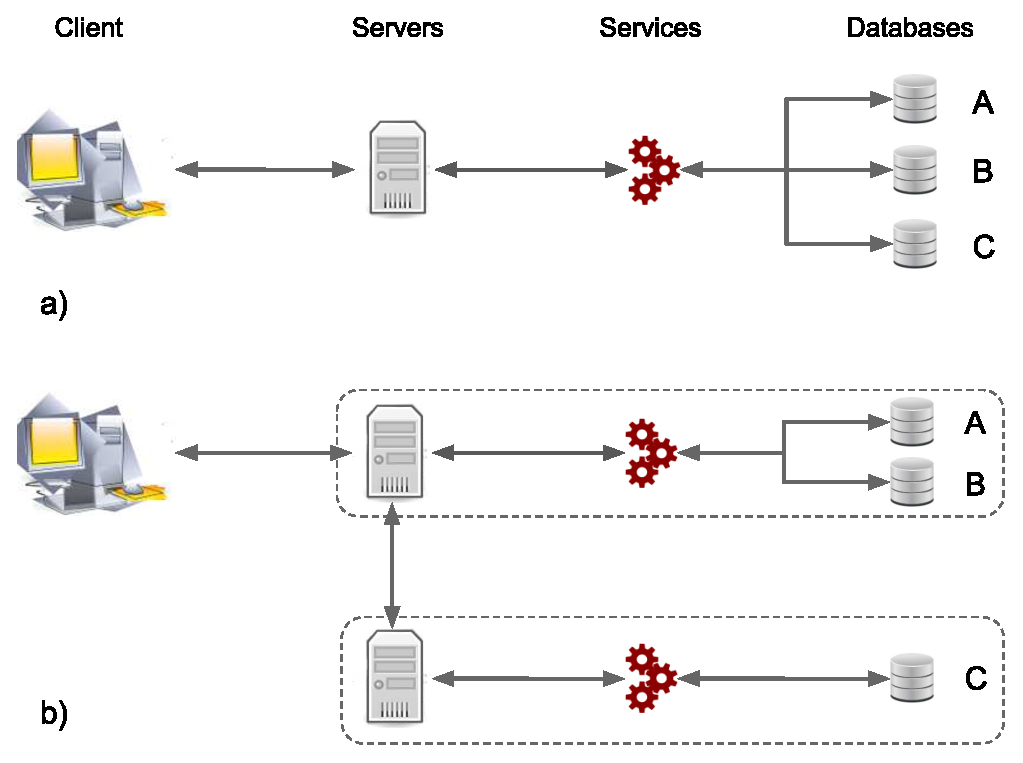
\includegraphics[width=\textwidth]{Grassroots_architecture}
\caption{\label{fig:client_view}A user's view of how a distributed service is called is shown in (a) with the actual cross-server communication shown in (b).}
\end{figure}

\begin{figure}[ht]
\centering
\begin{lstlisting}[style=json]
{
	"schema_version": 0.1,
	"provider": {
		"so:name": "Agris",
		"so:description": "A service to search for academic articles.",
		"so:url": "http://agris.fao.org/agris-search/index.do"
	},
	"services": {
		"path": "Agris Search service",
		"summary": "A service to obtain articles",
		"description": "A service to obtain articles using search terms",    
		"plugin": "web_search_service",
		"operations": [{
			"operation_id": "Agris Web Search service",
			"summary": "An operation to obtain matching articles",
			"so:description": "An operation to obtain matching articles from Agris",
			"about_uri": "http://agris.fao.org/agris-search/index.do",
			"uri": "http://agris.fao.org/agris-search/searchIndex.do",
			"method": "GET",
			"link_selector": "li.result-item h3 a",
			"parameter_set": {
				"parameters": [{
					"param": "query",
					"so:name": "Query",
					"default_value": "",
					"current_value": "",
					"type": "string",
					"grassroots_type": "params:keyword",
					"so:description": "The search term"
				}]
			}
		}]
	}
}
\end{lstlisting}
\caption{\label{fig:json_service}The JSON definition for wrapping a RESTful web service into a Grassroots service.}
\end{figure}

\begin{figure}[ht]
\centering
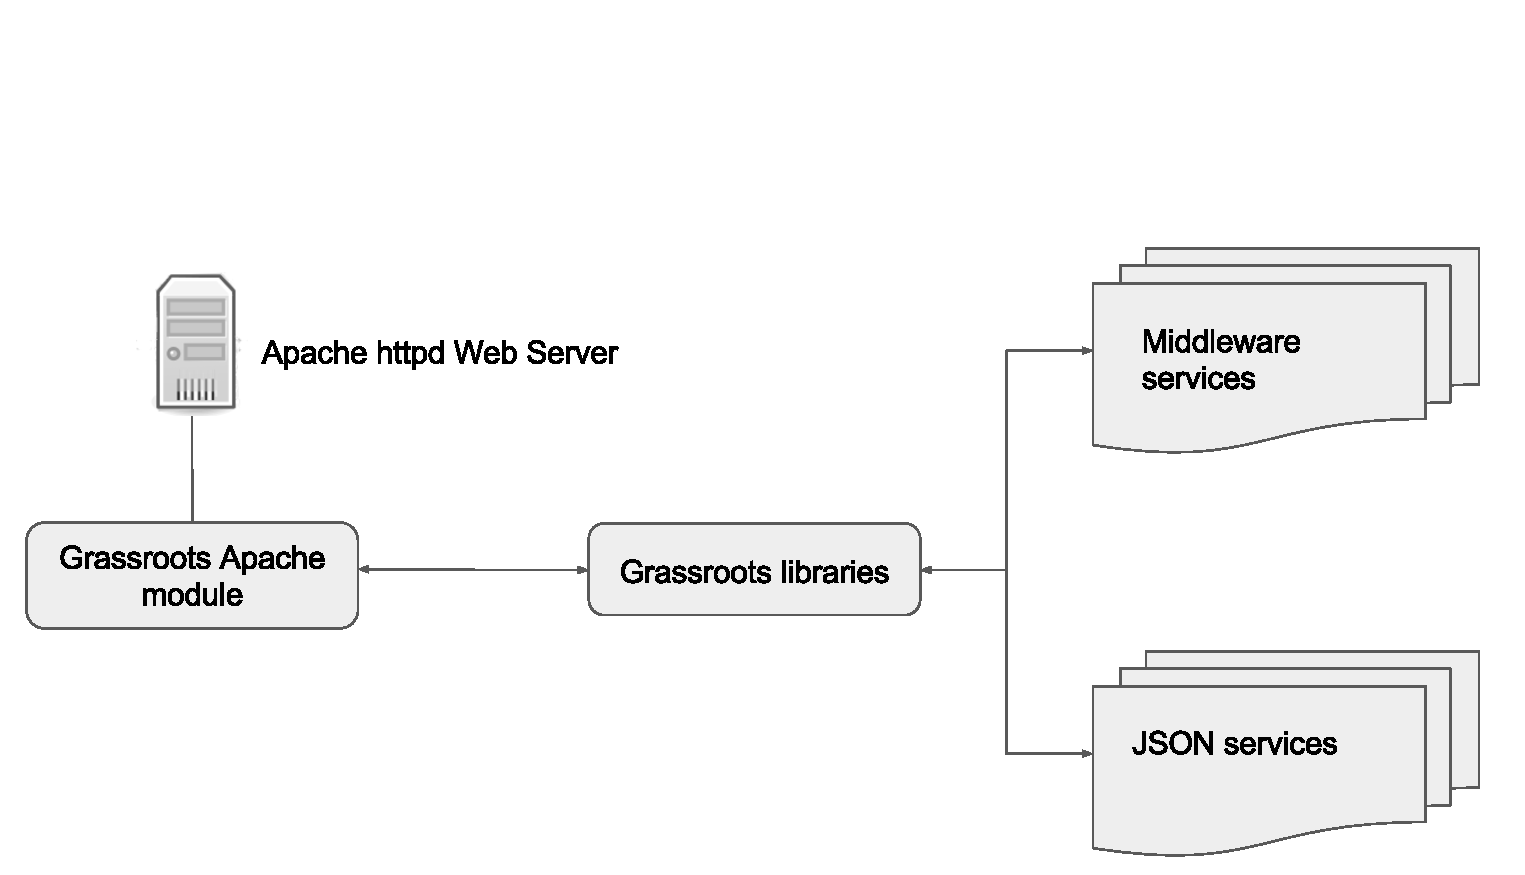
\includegraphics[width=\textwidth]{apache_grassroots}
\caption{\label{fig:httd_grassroots} The integration of Grassroots with httpd.}
\end{figure}


\begin{figure}[ht]
\centering
\begin{lstlisting}[style=json]
{
  "enum": [
    { "so:description": "Use Raw", "value": "z" },
    { "so:description": "Use Zip", "value": "zip" },
    { "so:description": "Use GZip", "value": "gz" }
  ]
}
\end{lstlisting}
\caption{\label{fig:parameter_enum}An example JSON fragment showing the list of valid values for a parameter.}
\end{figure}

% \subsection*{Mathematics}

% \LaTeX{} is great at typesetting mathematics. Let $X_1, X_2, \ldots, X_n$ be a sequence of independent and identically distributed random variables with $\text{E}[X_i] = \mu$ and $\text{Var}[X_i] = \sigma^2 < \infty$, and let
% $$S_n = \frac{X_1 + X_2 + \cdots + X_n}{n}
%       = \frac{1}{n}\sum_{i}^{n} X_i$$
% denote their mean. Then as $n$ approaches infinity, the random variables $\sqrt{n}(S_n - \mu)$ converge in distribution to a normal $\mathcal{N}(0, \sigma^2)$.

% \subsection*{Lists}

% You can make lists with automatic numbering \dots

% \begin{enumerate}
% \item Like this,
% \item and like this.
% \end{enumerate}
% \dots or bullet points \dots
% \begin{itemize}
% \item Like this,
% \item and like this.
% \end{itemize}

% See this guide for more information on BibTeX:
% http://libguides.mit.edu/content.php?pid=55482&sid=406343

% For more author guidance please see:
% http://f1000research.com/author-guidelines


% When all authors are happy with the paper, use the 
% ‘Submit to F1000RESEARCH' button from the menu above
% to submit directly to the open life science journal F1000Research.

% Please note that this template results in a draft pre-submission PDF document.
% Articles will be professionally typeset when accepted for publication.

% We hope you find the F1000Research Overleaf template useful,
% please let us know if you have any feedback using the help menu above.


\end{document}